\documentclass[journal,12pt,twocolumn]{IEEEtran}

\usepackage{setspace}
\usepackage{gensymb}

\singlespacing


\usepackage[cmex10]{amsmath}

\usepackage{amsthm}

\usepackage{mathrsfs}
\usepackage{txfonts}
\usepackage{stfloats}
\usepackage{bm}
\usepackage{cite}
\usepackage{cases}
\usepackage{subfig}

\usepackage{longtable}
\usepackage{multirow}

\usepackage{enumitem}
\usepackage{mathtools}
\usepackage{steinmetz}
\usepackage{tikz}
\usepackage{circuitikz}
\usepackage{verbatim}
\usepackage{tfrupee}
\usepackage[breaklinks=true]{hyperref}
\usepackage{graphicx}
\usepackage{tkz-euclide}
\usepackage{float}

\usetikzlibrary{calc,math}
\usepackage{listings}
    \usepackage{color}                                            %%
    \usepackage{array}                                            %%
    \usepackage{longtable}                                        %%
    \usepackage{calc}                                             %%
    \usepackage{multirow}                                         %%
    \usepackage{hhline}                                           %%
    \usepackage{ifthen}                                           %%
    \usepackage{lscape}     
\usepackage{multicol}
\usepackage{chngcntr}

\DeclareMathOperator*{\Res}{Res}

\renewcommand\thesection{\arabic{section}}
\renewcommand\thesubsection{\thesection.\arabic{subsection}}
\renewcommand\thesubsubsection{\thesubsection.\arabic{subsubsection}}

\renewcommand\thesectiondis{\arabic{section}}
\renewcommand\thesubsectiondis{\thesectiondis.\arabic{subsection}}
\renewcommand\thesubsubsectiondis{\thesubsectiondis.\arabic{subsubsection}}


\hyphenation{op-tical net-works semi-conduc-tor}
\def\inputGnumericTable{}                                 %%

\lstset{
%language=C,
frame=single, 
breaklines=true,
columns=fullflexible
}
\begin{document}


\newtheorem{theorem}{Theorem}[section]
\newtheorem{problem}{Problem}
\newtheorem{proposition}{Proposition}[section]
\newtheorem{lemma}{Lemma}[section]
\newtheorem{corollary}[theorem]{Corollary}
\newtheorem{example}{Example}[section]
\newtheorem{definition}[problem]{Definition}

\newcommand{\BEQA}{\begin{eqnarray}}
\newcommand{\EEQA}{\end{eqnarray}}
\newcommand{\define}{\stackrel{\triangle}{=}}
\bibliographystyle{IEEEtran}
\providecommand{\mbf}{\mathbf}
\providecommand{\pr}[1]{\ensuremath{\Pr\left(#1\right)}}
\providecommand{\qfunc}[1]{\ensuremath{Q\left(#1\right)}}
\providecommand{\sbrak}[1]{\ensuremath{{}\left[#1\right]}}
\providecommand{\lsbrak}[1]{\ensuremath{{}\left[#1\right.}}
\providecommand{\rsbrak}[1]{\ensuremath{{}\left.#1\right]}}
\providecommand{\brak}[1]{\ensuremath{\left(#1\right)}}
\providecommand{\lbrak}[1]{\ensuremath{\left(#1\right.}}
\providecommand{\rbrak}[1]{\ensuremath{\left.#1\right)}}
\providecommand{\cbrak}[1]{\ensuremath{\left\{#1\right\}}}
\providecommand{\lcbrak}[1]{\ensuremath{\left\{#1\right.}}
\providecommand{\rcbrak}[1]{\ensuremath{\left.#1\right\}}}
\theoremstyle{remark}
\newtheorem{rem}{Remark}
\newcommand{\sgn}{\mathop{\mathrm{sgn}}}
\providecommand{\abs}[1]{\lvert#1\vert}
\providecommand{\res}[1]{\Res\displaylimits_{#1}} 
\providecommand{\norm}[1]{\lVert#1\rVert}
%\providecommand{\norm}[1]{\lVert#1\rVert}
\providecommand{\mtx}[1]{\mathbf{#1}}
\providecommand{\mean}[1]{E[ #1 ]}
\providecommand{\fourier}{\overset{\mathcal{F}}{ \rightleftharpoons}}
%\providecommand{\hilbert}{\overset{\mathcal{H}}{ \rightleftharpoons}}
\providecommand{\system}{\overset{\mathcal{H}}{ \longleftrightarrow}}
	%\newcommand{\solution}[2]{\textbf{Solution:}{#1}}
\newcommand{\solution}{\noindent \textbf{Solution: }}
\newcommand{\cosec}{\,\text{cosec}\,}
\providecommand{\dec}[2]{\ensuremath{\overset{#1}{\underset{#2}{\gtrless}}}}
\newcommand{\myvec}[1]{\ensuremath{\begin{pmatrix}#1\end{pmatrix}}}
\newcommand{\mydet}[1]{\ensuremath{\begin{vmatrix}#1\end{vmatrix}}}
\numberwithin{equation}{subsection}
\makeatletter
\@addtoreset{figure}{problem}
\makeatother
\let\StandardTheFigure\thefigure
\let\vec\mathbf
\renewcommand{\thefigure}{\theproblem}
\def\putbox#1#2#3{\makebox[0in][l]{\makebox[#1][l]{}\raisebox{\baselineskip}[0in][0in]{\raisebox{#2}[0in][0in]{#3}}}}
     \def\rightbox#1{\makebox[0in][r]{#1}}
     \def\centbox#1{\makebox[0in]{#1}}
     \def\topbox#1{\raisebox{-\baselineskip}[0in][0in]{#1}}
     \def\midbox#1{\raisebox{-0.5\baselineskip}[0in][0in]{#1}}
\vspace{3cm}
\title{ASSIGNMENT-6}
\author{Unnati Gupta}
\maketitle
\newpage
\bigskip
\renewcommand{\thefigure}{\theenumi}
\renewcommand{\thetable}{\theenumi}
Download all python codes from 
\begin{lstlisting}
https://github.com/unnatigupta2320/Assignment_6/blob/master/codes.py
\end{lstlisting}
%
and latex-tikz codes from 
%
\begin{lstlisting}
https://github.com/unnatigupta2320/Assignment_6
\end{lstlisting}
%
\section{Question No-2.105 ( quadforms)}
Find the area enclosed by the parabola $4y=3x^2$ and the line $\myvec{-3&2}\vec{x}=12$.
%
\section{Solution}
\begin{enumerate}
\item Given equation of parabola is:
\begin{align}
 4y&=3x^2
 \\
 3x^2-4y&=0
 \\
 x^2-\frac{4}{3}y&=0
\end{align}
\item Comparing with the standard equation :
\begin{align}
\vec{x}^T\vec{V}\vec{x}+2\vec{u}^T\vec{x}+f=0 \label{eq1}
\\
\vec{V}=\myvec{1&0\\0&0},\vec{u}=\myvec{0\\-\frac{2}{3}},f=0 
\end{align}
\item We can find the eigen values corresponding to the $\vec{V}$,
\begin{align}
\abs{\vec{V} - \lambda\vec{I}} = \mydet{1-\lambda & 0 \\ 0 & -\lambda} &= 0
\\
\implies (1- \lambda)(-\lambda) &= 0
\end{align}
$\therefore$ Eigen values are 
\begin{align}
\lambda_1 = 0 , \lambda_2 = 1
\end{align}
\item Calculating the eigen vectors corresponding to $\lambda_1 = 0 , \lambda_2 = 1$ respectively.
\begin{align}
\vec{V}\vec{x} &= \lambda\vec{x}
\\
\myvec{1 & 0 \\ 0 & 0}\vec{x} &=0 \implies \vec{p_1} = \myvec{0 \\ 1}
\\
\myvec{0 & 0 \\ 0 & -1}\vec{x} &=\vec{x}  \implies \vec{p_2} = \myvec{1 \\ 0}
\end{align}
\item By eigen decomposition on $\vec{V}$,
\begin{align}
\vec{V}=\vec{P}\vec{D}\vec{P}^T
\end{align}
Where,
\begin{align}
\vec{P} &= \myvec{\vec{p_1} & \vec{p_2}} = \myvec{0 & 1 \\ 1 & 0}
\\
\vec{D} &= \myvec{\lambda_1 & 0 \\ 0 & \lambda_2} =\myvec{0 & 0 \\ 0 & 1} 
\end{align}
\item To find the vertex of the parabola ,
\begin{align} \myvec{\vec{u^T}+\eta\vec{p_1^T}\\\vec{V} }\vec{c} &= \myvec{\vec{-f}\\\eta \vec{p_1} -\vec{u}}
\\
\text{where, }  \eta = \vec{u^T}\vec{p_1} = \frac{-2}{3}
\\
\implies\myvec{0 & \frac{-4}{3}\\1 & 0 \\0 & 0} \vec{c}&= \myvec{0\\0\\0}
\end{align}
\item The above equation implies that,
\begin{align}    
   \vec{c} &= \myvec{0 \\ 0}
\end{align}
\item To find the point of intersection:
\begin{itemize}
    \item Let $\vec{K}$ and $\vec{L}$ are point of intersection.
    \item The given line is:
\begin{align} 
\myvec{-3&2}\vec{x}=12
\\
\text{or, }2y=3x+12 \label{eq2}
\end{align}
\begin{align}
\therefore \vec{x}=\myvec{x\\\frac{12+3x}{2}} \text{satisfies it.}\label{eq3}   
\end{align}
\item From \eqref{eq1} we have:
\begin{align}
    \vec{x}^T\vec{V}\vec{x}+2\vec{u}^T\vec{x}+f=0
    \\
    \vec{x}^T\myvec{1&0\\0&0}\vec{x}+2\myvec{0&\frac{-2}{3}}\vec{x}+0=0
    \end{align}
\item Putting \eqref{eq3} in above equation we get:
\begin{align}
    \myvec{x&\frac{12+3x}{2}}\myvec{1&0\\0&0}\myvec{x\\\frac{12+3x}{2}}+\myvec{0&\frac{-4}{3}}\myvec{x\\\frac{12+3x}{2}}=0
    \end{align}
    \begin{align}
    &\implies x\myvec{x\\\frac{12+3x}{2}}+\myvec{0&\frac{-4}{3}}\myvec{x\\\frac{12+3x}{2}}=0
    \\
    &\implies x^2+\frac{\brak{-4}}{3}\brak{\frac{12+3x}{2}}=0
    \\
    &\implies x^2-2x-8=0
    \\
    &\implies x=-2,4
\end{align}
\item Putting values of x in \eqref{eq2}, we get:
\begin{align}
\text{When x = -2}\implies y&=3
\\
\implies \vec{K}&= \myvec{-2\\3}  
\\
\text{When x = 4},\implies y&=12
\\
\implies \vec{L}&= \myvec{4\\12}
\end{align}
\end{itemize}
\item For finding area enclosed by parabola and line:
  Area required,
\begin{align}
   A&= \text{Area under line} - \text{Area under parabola}
     \\
   A&= Ar(KLMNK)-Ar(KCLMCNK)
    \\
    A&= A_1 -A_2 \label{eqAREA}
    \end{align}
\item For finding area under the line that is $A_1$-
\textbf{KLMN} is a trapezium. So its area can be given as:
\begin{align}
  A_1 &= MN\times\frac{\brak{KN+ML}}{2} 
  \\
   A_1 &= 6\times\frac{\brak{3+12}}{2} 
   \\
    A_1 &=45 \text{ units} \label{eqB}
\end{align}
\item For finding area under the parabola that is $A_2$-
\begin{align}
    A_2&= \int_{-2}^{4} y dx
    \\
    A_2&= \int_{-2}^{4} \frac{3}{4} x^2 dx
    \\
    A_2&= \frac{3}{4} \int_{-2}^{4}  x^2 dx
    \\
    A_2&= \frac{3}{4\times3} \brak{4^3-\brak{-2}^3}
    \\
    A_2&= \frac{1}{4} \brak{64 +8}
    \\
    A_2&= \frac{72}{4} 
    \\
    A_2&= 18 \text{ units} \label{eqC}
\end{align}
\item Putting \eqref{eqB} and \eqref{eqC} in \eqref{eqAREA} we get required area A as:
\begin{align}
 A &= A_1 -A_2 
 \\
 A &= 45-18
 \\
 A &= 27 \text{ units}
\end{align}
So, the required area A is \textbf{27 units}
\numberwithin{figure}{section}
\begin{figure}[ht]
\centering
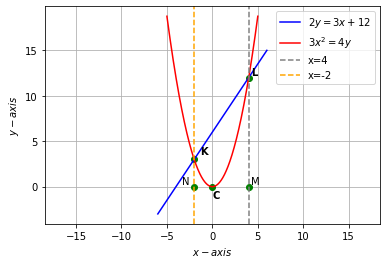
\includegraphics[width=\columnwidth]{Parabola-Line.png}
\caption{Plot of the parabola and line}
\label{Plot of the Parabola and line}
\end{figure}
\end{enumerate}
\end{document}
